\documentclass[12pt]{report}

% Paquetes LaTeX y estilos globales
\usepackage{multicol}
\usepackage{xcolor}
\usepackage{subfigure}
\usepackage[spanish]{babel}
\usepackage[utf8]{inputenc}
\usepackage{graphicx}
\usepackage{tabularx}
\usepackage{array}
\usepackage{titlesec}
\usepackage{xurl}
\usepackage[bookmarks,breaklinks,colorlinks=true,allcolors=blue]{hyperref}
\usepackage{listings}
\usepackage{inconsolata}
\usepackage{float}
\usepackage{eso-pic}
\usepackage[framemethod=tikz]{mdframed}

\usepackage[square,numbers]{natbib}
\AtBeginDocument{
  \renewcommand{\bibsection}{\chapter{\bibname}}
} % Bibliografia en capitulo numerado

\usepackage{geometry}
\usepackage{amsmath}
\usepackage{parskip}
\usepackage[official]{eurosym}
\usepackage{csquotes}

\input{etc/style}

% Comienzo del documento
\begin{document}

    % Portada y secciones no numeradas
    \begin{center}

\vspace*{1cm}

%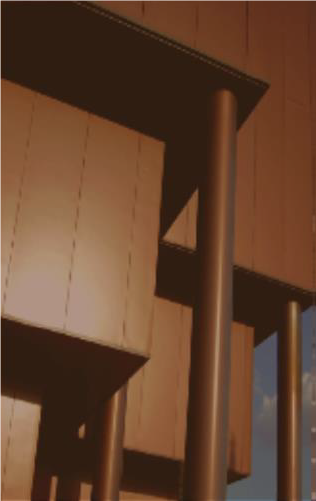
\includegraphics[width=0.25\textwidth]{fig/ilustracion.png}

\includegraphics[width=0.4\textwidth]{fig/miscdg-2.png}

%{\color{US_red} \rule{\linewidth}{0.75mm} }


\vspace*{2cm}
\begin{large}
TRABAJO FIN DE MÁSTER
\end{large}

\vspace*{0.1in}
%Versión en amarillo
\AddToShipoutPictureBG*{\AtPageLowerLeft{%
  \color{US_red!20}\rule{.25\paperwidth}{\paperheight}}}
%versión en rojo
%\AddToShipoutPictureBG*{\AtPageLowerLeft{% \color{US_red!20}\rule{.3\paperwidth}{\paperheight}}}
  
\textbf{\huge Título del trabajo} % Aquí el título de su trabajo

\vspace*{.2in}

{\large Realizado por}\\
\textbf{\Large Sergio Álvarez Piñón} % Aquí su nombre

\vspace*{2cm}
\begin{mdframed}[style=US_style]
\centering
\textbf{Para la obtención del título de}\\
{\large Máster en Ingeniería del Software: Cloud, Datos y Gestión TI} 

\vspace*{0.2in}

\textbf{Dirigido por}\\
{\large José María Luna Romera}\\ % Repetir esta línea si hay más de un tutor

\vspace*{0.2in}
\end{mdframed}


\vspace*{.6in}
\textbf{Convocatoria de Junio, curso 2025/26} % Adaptar al curso en el que presente el trabajo
\vspace*{0.2in}
\end{center}


\thispagestyle{empty} % Impide que se incluya número de página en la portada
\clearpage\setcounter{page}{1} % Comienza a incluir números de página a partir de aquí
\pagenumbering{roman} % En números romanos
    \chapter*{Agradecimientos}
A Paula, por tu apoyo incondicional durante estos meses. Sin ti, este camino habría sido mucho más duro.
    \chapter*{Resumen}

Este Trabajo Fin de Máster aborda la clasificación binaria de música de origen humano frente a música generada mediante inteligencia artificial, en el ámbito de la detección de música sintética. Su objetivo es comparar un enfoque clásico basado en MFCC y SVM con núcleo RBF y un enfoque profundo basado en MERT-v1-95M congelado y SVM lineal. El estudio utiliza AIME y un subconjunto equilibrado de 1\,000 ejemplos, 500 humanos y 500 generados mediante IA, evaluando ambos enfoques bajo el mismo protocolo experimental.

En el conjunto de \textit{test}, MFCC + SVM obtuvo una \textit{balanced accuracy} de 0,8333 y un ROC-AUC de 0,9086, frente a 0,8200 y 0,8985 de MERT + SVM, respectivamente. Los resultados fueron próximos, aunque MFCC presentó una ligera ventaja global en las métricas finales. Por ello, MFCC + SVM RBF se seleccionó para la prueba de concepto web por el compromiso entre rendimiento predictivo y menor complejidad operacional. Finalmente, el modelo seleccionado se integró y desplegó en VeriSon como una aplicación web funcional para el análisis de archivos de audio.

\vspace{.5cm}

\textbf{Palabras clave:} música generada por inteligencia artificial, detección de música sintética, clasificación de audio, MFCC, SVM, MERT, AIME.
    \chapter*{Abstract}

This Master's Thesis addresses the binary classification of human-origin music versus music generated using artificial intelligence, within the field of synthetic music detection. Its objective is to compare a classical approach based on MFCC and an RBF-kernel SVM with a deep approach based on frozen MERT-v1-95M representations and a linear SVM. The study uses AIME and a balanced subset of 1,000 examples, with 500 human and 500 AI-generated samples, evaluating both approaches under the same experimental protocol.

On the test set, MFCC + SVM achieved a \textit{balanced accuracy} of 0.8333 and a ROC-AUC of 0.9086, compared with 0.8200 and 0.8985 for MERT + SVM, respectively. The results were close, although MFCC showed a slight overall advantage in the final metrics. Therefore, MFCC + SVM RBF was selected for the web proof of concept due to its balance between predictive performance and lower operational complexity. Finally, the selected model was integrated and deployed in VeriSon as a functional web application for audio file analysis.

\vspace{.5cm}

\textbf{Keywords:} AI-generated music, synthetic music detection, audio classification, MFCC, SVM, MERT, AIME.
    
    % Índice del documento y de figuras
    \begingroup
        % Los enlaces son normalmente azules, pero en los índices se configuran a negro
        % para que no aparezca todo azul
        \hypersetup{linkcolor=black}
        \tableofcontents
        \listoffigures
        \lstlistoflistings
    \endgroup
    
    % Cambia el estilo de números de página a normal
    \clearpage\pagenumbering{arabic}
    
    % Capítulos del trabajo
    \chapter{Introducción}
\label{cap:introduccion}

\section{Introducción}
\label{sec:introduccion:intro}
En los últimos años, la generación automática de música mediante inteligencia artificial ha experimentado un avance muy significativo. La aparición de modelos text-to-music y de servicios que permiten utilizarlos con facilidad ha hecho que estas tecnologías se extiendan más allá de entornos especializados. Sistemas como MusicGen, AudioLDM2 o Stable Audio Open, junto con plataformas comerciales como Suno y Udio, han contribuido a popularizar su uso tanto en entornos experimentales como en contextos reales.

Este progreso abre nuevas posibilidades creativas y productivas, pero también plantea retos importantes. A medida que la música generada por IA alcanza niveles de calidad cada vez mayores, resulta más difícil distinguir entre obras creadas por personas y contenido generado artificialmente. Esta situación no solo plantea un desafío técnico, sino que también afecta a cuestiones como la autenticidad del contenido, su trazabilidad y la protección de los derechos de autor. En este contexto, la detección de música generada por IA se ha convertido en un problema cada vez más relevante. Disponer de métodos capaces de identificar este tipo de contenido puede resultar útil en escenarios como plataformas de distribución, servicios de streaming, sistemas de recomendación, verificación de procedencia o análisis de copyright.

Para abordar este problema, se han propuesto distintos métodos de detección basados en técnicas de procesamiento de audio y aprendizaje automático. Sin embargo, la literatura reciente señala que, aunque algunos detectores ofrecen resultados prometedores en entornos controlados, todavía presentan limitaciones de generalización y robustez cuando cambian los generadores utilizados, el tipo de audio analizado o las transformaciones aplicadas a la señal. En particular, algunos estudios señalan que modificaciones aparentemente simples, como el resampling o determinadas alteraciones del audio, pueden degradar de forma notable el rendimiento de estos sistemas.

A partir de esta situación, el presente Trabajo Fin de Máster aborda el problema de la atribución cerrada del generador en música sintética desde una perspectiva comparativa y reproducible. En concreto, se propone diseñar e implementar un pipeline experimental común para evaluar diversas técnicas de representación de audio y diferentes modelos de clasificación bajo las mismas condiciones. Para ello, el trabajo se apoyará en un conjunto de datos de referencia utilizado en la literatura reciente y en varias combinaciones representativas de preprocesado, extracción de características y clasificación, con el objetivo de analizar qué enfoques ofrecen mejores resultados en la identificación del generador utilizado para crear una pieza musical sintética dentro de un mismo marco experimental.

\section{Contexto del TFM}
\label{sec:introduccion:contexto}
Desarrolle de forma razonada los siguientes puntos:
\begin {enumerate}
\item Grado de dificultad o complejidad del tema (Para contestar a esta pregunta, considere los siguientes factores: ¿se da solución a un problema no resuelto previamente? ¿Se usan tecnologías muy novedosas o poco estudiadas? ¿Se ha resuelto un problema haciendo uso de recursos limitados o muy reducidos en comparación con soluciones previas?):
\item Grado de cumplimiento de los objetivos planteados:
\item Componente de investigación del trabajo:
\item Potencial aplicación de este trabajo en un entorno académico o industrial:
\end{enumerate}


\section {Estructura de este documento}
\label{sec:introduccion:estructura}
El presente documento se estructura en los siguientes capítulos:
\begin{itemize}
    \item \textbf{Introducción:} presenta el contexto general del trabajo, el problema abordado, la motivación del TFM y la organización del documento.
    \item \textbf{Estudio previo:} recoge la definición del problema, los objetivos, la metodología de trabajo, la planificación temporal y el presupuesto estimado del proyecto.
    \item \textbf{Estado del arte:} revisa los trabajos más relevantes relacionados con la generación musical mediante IA, la detección y atribución de música sintética, los datasets disponibles, las técnicas de representación de audio y los modelos de clasificación empleados en la literatura.
    \item \textbf{Descripción de la propuesta:} describe la solución planteada en este TFM, incluyendo el dataset utilizado, el pipeline experimental, las técnicas de preprocesado, las representaciones de audio consideradas, los modelos implementados y el diseño de los experimentos de atribución cerrada.
    \item \textbf{Validación:} presenta las herramientas empleadas, los experimentos realizados, los resultados obtenidos y su análisis.
    \item \textbf{Conclusiones:} recoge las conclusiones finales del trabajo, sus limitaciones y las posibles líneas de trabajo futuro.
\end{itemize}
    \chapter{Estudio previo}
\label{cap:estudio-previo}

\section{Introducción}

Este capítulo define los objetivos del TFM y la metodología empleada para organizar el trabajo. El estudio se centra en una tarea de clasificación binaria entre música producida por humanos y música generada mediante IA, utilizando AIME como conjunto de datos principal y un protocolo experimental común para comparar los modelos.

La comparación incluye un enfoque clásico basado en MFCC + SVM y un único modelo profundo de audio preentrenado. La evaluación considera tanto el rendimiento predictivo como el comportamiento operacional, de forma que la selección del modelo tenga en cuenta su utilidad dentro de una prueba de concepto web.

\section{Objetivos}

\subsection{Objetivo general}

Comparar un enfoque clásico basado en MFCC y SVM con un modelo profundo preentrenado para la detección de música generada mediante inteligencia artificial, evaluando ambos mediante medidas predictivas y operacionales bajo un protocolo experimental común.

\subsection{Objetivos específicos}

\begin{enumerate}
    \item Revisar el estado del arte relacionado con la detección de música generada mediante IA.
    \item Auditar y preparar AIME para su uso experimental.
    \item Definir un protocolo reproducible de particionado, preprocesamiento y evaluación.
    \item Implementar y evaluar el baseline MFCC + SVM.
    \item Seleccionar, adaptar y evaluar un único modelo profundo preentrenado.
    \item Comparar ambos enfoques mediante medidas predictivas y operacionales, y seleccionar el modelo con mejor equilibrio entre rendimiento predictivo y coste operacional.
    \item Desarrollar y desplegar una prueba de concepto web que integre el modelo seleccionado.
    \item Documentar decisiones, experimentos y artefactos para garantizar la reproducibilidad.
\end{enumerate}

\section{Metodología}

El proyecto sigue un desarrollo iterativo e incremental organizado mediante fases, issues y ciclos de trabajo breves. Esta forma de trabajo permite dividir el TFM en tareas manejables, revisar los resultados de cada etapa y mantener trazabilidad entre decisiones, experimentos y artefactos generados.

\subsection{Documentación y revisión bibliográfica}

La memoria se redacta en LaTeX mediante Overleaf, manteniendo una estructura de capítulos coherente con los requisitos del TFM. La revisión bibliográfica se organiza de forma estructurada y trazable, de modo que las fuentes empleadas puedan relacionarse con las decisiones metodológicas y con el estado del arte descrito en la memoria.

\subsection{Gestión del proyecto y control de versiones}

El desarrollo se gestiona con Git y GitHub, utilizando ramas e issues para separar tareas y registrar cada bloque de trabajo. Las decisiones relevantes, los experimentos ejecutados y los artefactos producidos se documentan en el repositorio para facilitar su revisión posterior.

\subsection{Preparación de los datos y reproducibilidad}

La preparación experimental parte de la selección y auditoría de AIME como conjunto de datos principal. Antes del procesamiento de audio se generan particiones reproducibles, separando entrenamiento, validación y prueba. Esta separación permite controlar fugas de información y mantener el mismo conjunto de datos para evaluar los dos enfoques comparados.

\subsection{Desarrollo y evaluación experimental}

Los modelos se evalúan bajo el mismo protocolo experimental. La validación se utiliza para seleccionar configuraciones y el conjunto de prueba se reserva para la evaluación final. Durante el proceso se registran medidas predictivas y operacionales, y se incorporan pruebas automatizadas sobre los componentes críticos para comprobar que el particionado, el preprocesamiento y la evaluación respetan las condiciones definidas y no introducen fugas de información.

\section{Planificación}

\section{Presupuesto}

    \chapter{Estado del arte}
\label{cap:estado-arte}

\section{Introducción y delimitación del problema}

La detección de música generada mediante inteligencia artificial se ha ido consolidando como un problema propio dentro del análisis de audio. En trabajos recientes, esta tarea aparece bajo la denominación \textit{Synthetic Song Detection} (SSD), entendida como la clasificación entre canciones producidas por humanos y canciones generadas de extremo a extremo mediante sistemas de IA \cite{rahman2024sonics}.

Esta delimitación es importante porque existen tareas cercanas que conviene distinguir. La \textit{Singing Voice Deepfake Detection} se centra en detectar voces cantadas sintéticas o convertidas, a menudo dentro de mezclas donde el acompañamiento puede proceder de música real \cite{zang2023singfake,zang2024ctrsvdd}. La detección de canciones sintéticas de extremo a extremo, en cambio, considera que pueden ser artificiales la voz, la instrumentación, la letra, el arreglo y la producción global. SSD también se diferencia de la detección de voz hablada sintética, la detección de audio sintético general, la identificación de letras generadas mediante IA y la atribución del modelo generador.

El interés de SSD va más allá de obtener una decisión automática sobre un archivo de audio. La música es una señal con estructura temporal, patrones tímbricos, organización rítmica y relaciones de larga duración. Por ello, los detectores pueden apoyarse tanto en indicios locales de la señal como en propiedades musicales más amplias. Esta combinación explica que el campo incluya desde enfoques clásicos basados en características acústicas hasta modelos profundos que intentan aprovechar representaciones aprendidas y relaciones entre fragmentos.

\section{Conjuntos de datos para detección de música sintética}

En el contexto de SSD, SONICS aporta un conjunto de datos específico para detectar canciones generadas de extremo a extremo. Sus autores señalan que muchos corpus previos se centraban en voz cantada sintética, mientras que los sistemas actuales pueden generar también la instrumentación, el arreglo y la producción global \cite{rahman2024sonics}. Esta diferencia motiva la creación de conjuntos específicos para canciones completas y de protocolos capaces de considerar relaciones temporales más amplias.

FakeMusicCaps aborda un problema próximo desde otra perspectiva. El conjunto de datos se construye a partir de MusicCaps, regenerando pares música-texto mediante varios modelos \textit{text-to-music}. Además de la detección binaria, el trabajo estudia la atribución del modelo generador \cite{comanducci2024fakemusiccaps}. FakeMusicCaps constituye un ejemplo de corpus específico para música generada mediante IA y muestra cómo la detección puede verse condicionada por los generadores incluidos en el conjunto de datos.

AIME ocupa una posición distinta. La tarjeta oficial del conjunto de datos lo presenta como \textit{AI Music Evaluation Dataset}, con música generada por distintos modelos y ejemplos procedentes de MTG-Jamendo, junto con metadatos como el modelo de origen y una descripción basada en etiquetas \cite{discoethAIME}. Su finalidad original está vinculada a la evaluación de modelos de generación musical y preferencias humanas, por lo que su utilización en detección requiere definir y documentar un protocolo experimental propio \cite{groetschla2025benchmarking}.

La reutilización de AIME para detección cuenta al menos con un antecedente verificado: \textit{Fusion Segment Transformer}, identificado como preprint de 2026, evalúa su propuesta en SONICS y AIME \cite{kim2026fusionsegmenttransformer}. Esta evidencia es todavía limitada, aunque muestra que el corpus puede emplearse en trabajos de detección cuando se explicita el protocolo experimental.

\section{Enfoques clásicos con características acústicas}

Los enfoques clásicos de clasificación de audio suelen partir de características acústicas calculadas manualmente. Estas representaciones resumen propiedades de la señal antes de aplicar un clasificador, lo que permite construir sistemas relativamente simples, reproducibles y de bajo coste computacional. En este contexto, los MFCC representan información espectral de corto plazo mediante vectores compactos.

Los MFCC se han utilizado en tareas relacionadas de detección de audio sintético, especialmente en sistemas de anti-\textit{spoofing} de voz. El precedente aplicado citado en este capítulo es Novoselov et al., que emplean MFCC dentro del reto ASVspoof 2015 y comparan clasificadores clásicos con enfoques más complejos \cite{novoselov2015stcantispoofing}. Aunque este dominio no coincide con SSD, sirve como antecedente metodológico para entender su uso como representación acústica compacta en problemas de detección.

La SVM es un clasificador clásico para tareas supervisadas, especialmente adecuado cuando se trabaja con vectores de características fijas. Su formulación de margen máximo y el uso de kernels permiten construir fronteras de decisión no lineales sin requerir arquitecturas profundas \cite{cortes1995support}. La combinación MFCC + SVM constituye un baseline clásico reproducible y controlable, basado en características acústicas compactas.

La principal limitación de este tipo de aproximación es que resume la señal en descriptores compactos. Esto puede ser suficiente para capturar ciertos patrones espectrales, pero deja menos margen para modelar relaciones temporales largas, estructura musical o dependencias entre secciones de una canción. Estas limitaciones han favorecido el estudio de representaciones profundas capaces de modelar información acústica y temporal más compleja.

\section{Enfoques profundos y representaciones preentrenadas}

El desarrollo reciente de SSD se ha desplazado hacia modelos profundos capaces de aprender representaciones más ricas a partir del audio. SONICS propone SpecTTTra, una arquitectura orientada a capturar dependencias temporales largas con menor coste que algunos modelos convolucionales o transformadores de referencia \cite{rahman2024sonics}. Esta línea pone de manifiesto que la detección de canciones completas depende tanto de indicios locales como de la forma en que la música se organiza a lo largo del tiempo.

Otra línea dentro de los enfoques profundos consiste en reutilizar conocimiento aprendido previamente, en lugar de entrenar toda la arquitectura desde cero para el problema concreto. Los encoders de audio pueden entrenarse sobre corpus amplios y después emplearse como extractores de vectores para tareas de clasificación.

Dentro de esta línea se sitúa MERT, entrenado mediante aprendizaje autosupervisado a gran escala sobre audio musical \cite{li2024mert}. Su propuesta combina objetivos acústicos y de alto nivel durante el preentrenamiento para capturar información reutilizable. Los vectores resultantes se evaluaron en problemas de recuperación y comprensión de información musical, lo que sitúa a MERT como un encoder especializado en este dominio.

\section{Segmentación y evaluación a nivel de canción}

La segmentación aparece de forma natural en detección musical porque las canciones pueden tener duraciones superiores a las que muchos modelos procesan directamente. Trabajar con fragmentos permite adaptar el audio a modelos con entradas de duración fija, acotar el coste de cada inferencia y obtener varias observaciones de una misma pieza. La decisión a nivel de canción requiere, además, una estrategia de agregación adecuada.

Segment Transformer divide el audio en segmentos, extrae información de cada uno mediante modelos preentrenados o autosupervisados y aprende relaciones entre fragmentos para mejorar la detección a escala de canción \cite{kim2025segmenttransformer}. La propuesta muestra la utilidad de separar el análisis local de los fragmentos y el modelado estructural posterior, especialmente cuando el audio completo es demasiado largo para tratarse de una sola vez.

El preprint \textit{Fusion Segment Transformer} amplía esta idea mediante una fusión guiada de información de contenido y estructura, y proporciona una evidencia directa de evaluación sobre AIME dentro de un trabajo de detección \cite{kim2026fusionsegmenttransformer}. Esta línea refuerza la relevancia de los enfoques por segmentos en problemas de detección musical.

En tareas de clasificación musical, la forma de dividir el audio y agregar predicciones puede afectar a las medidas de rendimiento. Nasrullah y Zhao muestran, en clasificación de artistas, que la longitud de los fragmentos, el esquema de particionado y la agregación a nivel de canción influyen en la evaluación \cite{nasrullah2019musicartistclassification}. Aunque la tarea es distinta, el resultado es relevante para diseñar protocolos de segmentación que eviten la mezcla de información relacionada entre particiones.

Los trabajos específicos de SSD también refuerzan esta idea. SONICS destaca la importancia de las dependencias de larga duración, mientras que Segment Transformer modela explícitamente relaciones entre segmentos \cite{rahman2024sonics,kim2025segmenttransformer}. Esto sugiere que un detector puede operar sobre fragmentos y, al mismo tiempo, necesitar una estrategia de agregación si se desea emitir una decisión sobre una canción completa.

\section{Generalización, robustez y limitaciones actuales}

Una dificultad recurrente en SSD es la generalización fuera del escenario de entrenamiento. Afchar et al. muestran que obtener una medida alta en una prueba cerrada resulta insuficiente para considerar resuelto el problema, ya que la robustez frente a manipulaciones del audio y la generalización a generadores no vistos siguen siendo cuestiones críticas \cite{afchar2025challenges}. Esta advertencia es especialmente importante cuando los detectores pueden aprender atajos acústicos asociados a un conjunto de datos, a un códec o a un proceso de producción concreto.

Los cambios de dominio también aparecen en trabajos adyacentes de SVDD. SingFake identifica dificultades con cantantes no vistos, códecs de comunicación, idiomas y contextos musicales \cite{zang2023singfake}. CtrSVDD, por su parte, destaca que la selección de características y la separación entre métodos de falsificación vistos y no vistos afectan al comportamiento del detector \cite{zang2024ctrsvdd}. Aunque pertenecen a una tarea distinta, estos resultados muestran la fragilidad de los detectores cuando cambian las condiciones de evaluación.

Los preprints recientes de 2026 insisten en esa misma dirección desde la detección de música generada mediante IA. MusicDET plantea explícitamente la detección ante generadores no vistos mediante un enfoque \textit{zero-shot} \cite{han2026musicdet}. Broadcast Monitoring analiza un escenario donde la música aparece en fragmentos cortos o enmascarada por habla, y muestra que las condiciones de emisión pueden degradar modelos entrenados para contextos más limpios \cite{lopezayala2026broadcast}. ArtifactNet, también como preprint, centra la atención en la robustez frente a códecs y en detectores ligeros basados en residuos forenses \cite{oh2026artifactnet}.

En conjunto, estas aportaciones muestran que las medidas obtenidas en un corpus cerrado deben interpretarse con cautela. La duración de los fragmentos, el idioma, el artista, el género, la frecuencia de muestreo, la compresión y los artefactos de producción pueden influir en la decisión del modelo. Por tanto, una comparación experimental rigurosa debe distinguir entre rendimiento dentro del conjunto de datos evaluado y capacidad de generalización a condiciones externas.

\section{Conclusiones}

Synthetic Song Detection es una tarea reciente y todavía en desarrollo. Aunque ya existen conjuntos de datos y arquitecturas específicas para música generada de extremo a extremo, todavía falta un enfoque consolidado que pueda considerarse solución general. Los resultados en escenarios cerrados son útiles para comparar modelos, pero ofrecen garantías limitadas ante nuevos generadores, transformaciones de audio o cambios de dominio.

La revisión realizada permite justificar la comparación entre un enfoque basado en MFCC y SVM y un enfoque profundo basado en MERT congelado y SVM bajo condiciones comunes de evaluación. El primero aporta una referencia reproducible basada en características manuales, mientras que el segundo permite evaluar representaciones profundas preentrenadas orientadas al dominio musical.

Por último, AIME debe presentarse con precisión: es un corpus documentado procedente de la evaluación de modelos de generación musical, reutilizado aquí para detección binaria tras una auditoría propia. La clase IA incluye doce generadores, lo que evita depender de un único generador dentro del corpus, aunque no garantiza generalización a generadores o datasets no vistos.

    \chapter{Descripción de la propuesta}\label{cap:diseño}

\section{Introducción}
En este capítulo explicaremos...

\section{Conclusiones}
En este capítulo concluimos que...
    \chapter{Validación}\label{cap:validacion}

\section{Introducción}

Este capítulo presenta la validación experimental de los dos enfoques implementados: el baseline clásico MFCC + SVM y el enfoque profundo basado en MERT congelado y SVM. Se recogen la ejecución de los experimentos, la selección de configuraciones, la evaluación final en \textit{test}, la comparación predictiva y operacional, y la selección del modelo para la prueba de concepto web.

\section{Baseline MFCC + SVM}

\subsection*{Configuración y selección}

El baseline procesó los 1\,000 ejemplos del manifiesto experimental sin registrar fallos.

La búsqueda de hiperparámetros evaluó 16 configuraciones de SVM RBF, combinando $C \in \{0{,}1;\ 1;\ 10;\ 100\}$ y $\gamma \in \{\textit{scale};\ 0{,}001;\ 0{,}01;\ 0{,}1\}$. La configuración seleccionada fue $C=10$ y $\gamma=0{,}01$, ajustada con \textit{train} y seleccionada con \textit{val}.

\subsection*{Resultados}

\begin{table}[H]
    \centering
    \resizebox{\textwidth}{!}{%
    \begin{tabular}{lrrrrr}
        \hline
        \textbf{Partición} & \textbf{Balanced accuracy} & \textbf{Precision IA} & \textbf{Recall IA} & \textbf{F1 IA} & \textbf{ROC-AUC} \\
        \hline
        \textit{val} & 0,7800 & 0,7625 & 0,8133 & 0,7871 & 0,8480 \\
        \textit{test} & 0,8333 & 0,8472 & 0,8133 & 0,8299 & 0,9086 \\
        \hline
    \end{tabular}
    }
    \caption{Medidas predictivas del baseline MFCC + SVM en \textit{val} y \textit{test}.}
    \label{tab:mfcc-svm-resultados}
\end{table}

En \textit{test}, el baseline obtiene 125 aciertos sobre 150 ejemplos. La matriz de confusión muestra que clasifica correctamente 64 de los 75 ejemplos humanos y 61 de los 75 ejemplos IA, con 11 falsos positivos y 14 falsos negativos. Esta distribución indica una dificultad ligeramente mayor para reconocer la clase IA, coherente con un recall humano de 0,8533 y un recall IA de 0,8133. La Figura~\ref{fig:mfcc-svm-confusion} recoge esta distribución de aciertos y errores.

\begin{figure}[H]
    \centering
    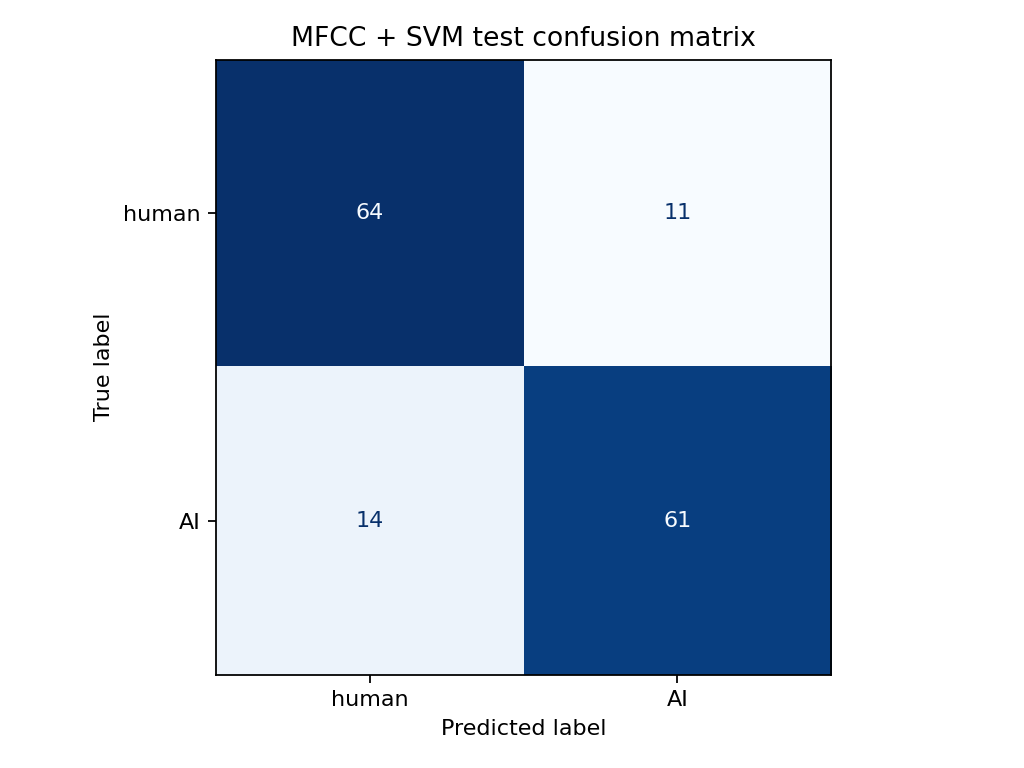
\includegraphics[width=0.72\textwidth]{fig/mfcc_svm_confusion_matrix.png}
    \caption{Matriz de confusión del baseline MFCC + SVM en \textit{test}.}
    \label{fig:mfcc-svm-confusion}
\end{figure}

\section{MERT congelado + SVM}

\subsection*{Extracción de embeddings}

Antes de procesar el subconjunto completo se ejecutó un smoke test técnico en CPU. Esta prueba verificó las dimensiones de entrada y salida, la presencia de valores finitos, el determinismo de la extracción y la viabilidad de ejecución en CPU.

La extracción completa procesó los 1\,000 ejemplos del manifiesto sin fallos, IDs ausentes ni duplicados. Cada clip produjo un vector de 768 componentes y el conjunto completo quedó representado mediante una matriz de forma $(1000, 768)$. Los embeddings se almacenaron como float32 y sus metadatos se verificaron frente al manifiesto.

\subsection*{Selección del clasificador}

El clasificador sobre embeddings se construyó como un pipeline \textit{StandardScaler} + SVM. Se evaluaron candidatos con kernel lineal y RBF. Todos los candidatos se ajustaron con \textit{train} y se seleccionaron con \textit{val}. La regla de selección maximizó \textit{balanced accuracy}; en caso de empate, consideró ROC-AUC, F1 de la clase IA, menor latencia media de predicción y preferencia por kernel lineal. La configuración seleccionada fue una SVM lineal con $C=0{,}1$. Las medidas obtenidas por esta configuración en \textit{val} se recogen en la Tabla~\ref{tab:mert-svm-validacion}.

\begin{table}[H]
    \centering
    \resizebox{\textwidth}{!}{%
    \begin{tabular}{lrrrrr}
        \hline
        \textbf{Modelo} & \textbf{Balanced accuracy} & \textbf{Precision IA} & \textbf{Recall IA} & \textbf{F1 IA} & \textbf{ROC-AUC} \\
        \hline
        MERT + SVM lineal & 0,8667 & 0,8395 & 0,9067 & 0,8718 & 0,9218 \\
        \hline
    \end{tabular}
    }
    \caption{Medidas de \textit{val} del clasificador seleccionado sobre embeddings MERT.}
    \label{tab:mert-svm-validacion}
\end{table}

\subsection*{Resultados}

Una vez fijada la configuración mediante \textit{val}, el enfoque basado en MERT se evaluó en \textit{test} utilizando los embeddings precomputados y una SVM lineal con $C=0{,}1$. La Tabla~\ref{tab:mert-svm-test} recoge las medidas obtenidas.

\begin{table}[H]
    \centering
    \resizebox{\textwidth}{!}{%
    \begin{tabular}{lrrrrr}
        \hline
        \textbf{Modelo} & \textbf{Balanced accuracy} & \textbf{Precision IA} & \textbf{Recall IA} & \textbf{F1 IA} & \textbf{ROC-AUC} \\
        \hline
        MERT + SVM lineal & 0,8200 & 0,8158 & 0,8267 & 0,8212 & 0,8985 \\
        \hline
    \end{tabular}
    }
    \caption{Medidas de \textit{test} de MERT + SVM lineal.}
    \label{tab:mert-svm-test}
\end{table}

En \textit{test}, el enfoque basado en MERT obtuvo 123 aciertos sobre 150 ejemplos. Clasificó correctamente 61 de los 75 ejemplos humanos y 62 de los 75 ejemplos IA, con 14 falsos positivos y 13 falsos negativos. La distribución de errores entre ambas clases fue prácticamente equilibrada, como muestra la Figura~\ref{fig:mert-svm-confusion}.

\begin{figure}[H]
    \centering
    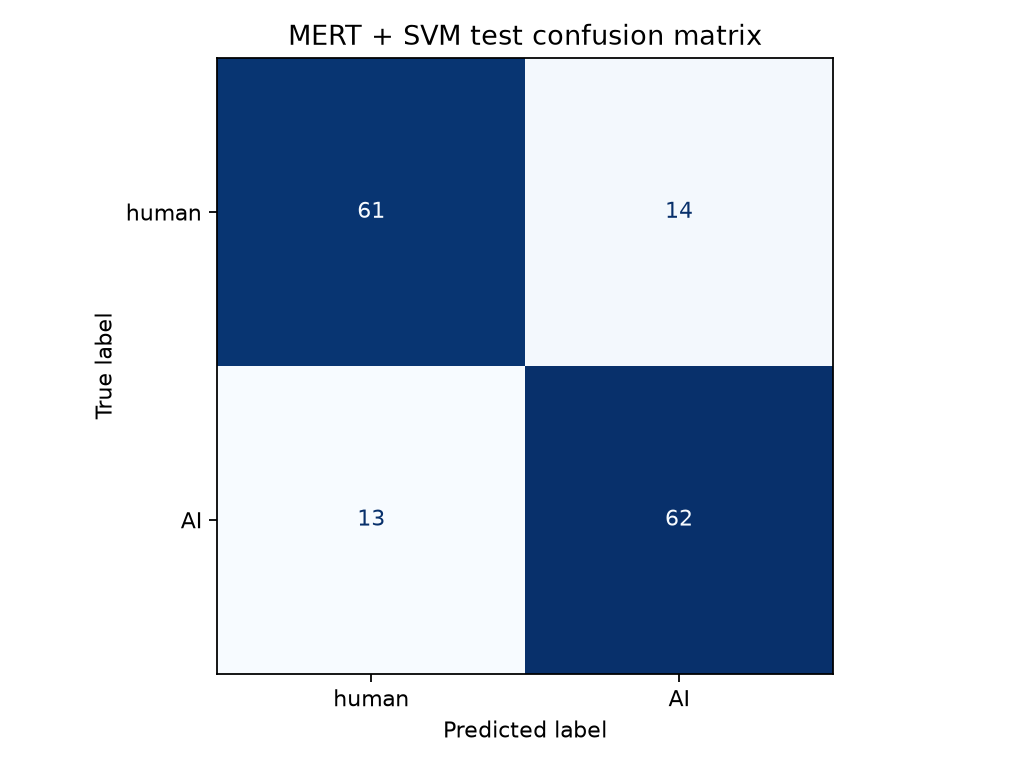
\includegraphics[width=0.72\textwidth]{fig/mert_svm_test_confusion_matrix.png}
    \caption{Matriz de confusión de MERT + SVM lineal en \textit{test}.}
    \label{fig:mert-svm-confusion}
\end{figure}

\section{Comparación y selección del modelo}

\subsection*{Comparación predictiva}

La Tabla~\ref{tab:comparacion-test} presenta las medidas de \textit{test} de ambos enfoques y la diferencia MERT menos MFCC.

\begin{table}[H]
    \centering
    \resizebox{\textwidth}{!}{%
    \begin{tabular}{lrrrrr}
        \hline
        \textbf{Modelo} & \textbf{Balanced accuracy} & \textbf{Precision IA} & \textbf{Recall IA} & \textbf{F1 IA} & \textbf{ROC-AUC} \\
        \hline
        MFCC + SVM RBF & 0,8333 & 0,8472 & 0,8133 & 0,8299 & 0,9086 \\
        MERT + SVM lineal & 0,8200 & 0,8158 & 0,8267 & 0,8212 & 0,8985 \\
        Diferencia MERT - MFCC & -0,0133 & -0,0314 & +0,0133 & -0,0087 & -0,0101 \\
        \hline
    \end{tabular}
    }
    \caption{Comparación predictiva en \textit{test}.}
    \label{tab:comparacion-test}
\end{table}

La Tabla~\ref{tab:comparacion-errores} compara los aciertos y errores principales de ambos enfoques.

\begin{table}[H]
    \centering
    \begin{tabular}{lrrr}
        \hline
        \textbf{Modelo} & \textbf{Aciertos} & \textbf{Falsos positivos} & \textbf{Falsos negativos} \\
        \hline
        MFCC + SVM RBF & 125 & 11 & 14 \\
        MERT + SVM lineal & 123 & 14 & 13 \\
        Diferencia MERT - MFCC & -2 & +3 & -1 \\
        \hline
    \end{tabular}
    \caption{Comparación de aciertos, falsos positivos y falsos negativos en \textit{test}.}
    \label{tab:comparacion-errores}
\end{table}

En \textit{test}, los resultados de ambos enfoques fueron próximos y deben interpretarse como comparables dentro de AIME. MFCC + SVM alcanzó una ligera ventaja en \textit{balanced accuracy}, precision IA, F1 IA y ROC-AUC, además de obtener 125 aciertos frente a los 123 del enfoque profundo. MERT + SVM presentó un recall IA ligeramente superior y un falso negativo menos. Dado el reducido tamaño de las diferencias observadas, estos resultados no permiten afirmar una superioridad estadísticamente significativa de MFCC sobre MERT. Las diferencias se circunscriben al \textit{test} de AIME empleado en el experimento.

\subsection*{Comparación operacional}

La comparación operacional de la Tabla~\ref{tab:comparacion-operacional} se refiere al clasificador aplicado sobre representaciones ya calculadas. En el baseline se usan características MFCC ya extraídas, mientras que en el enfoque profundo se usan embeddings MERT ya extraídos. El tamaño corresponde al clasificador serializado; en el caso de MERT no incluye el processor ni el encoder.

\begin{table}[H]
    \centering
    \begin{tabular}{lrr}
        \hline
        \textbf{Modelo} & \textbf{Latencia (ms/ejemplo)} & \textbf{Tamaño (MB)} \\
        \hline
        MFCC + SVM RBF & 0,090 & 0,14 \\
        MERT + SVM lineal & 0,113 & 1,69 \\
        \hline
    \end{tabular}
    \caption{Comparación operacional de los clasificadores.}
    \label{tab:comparacion-operacional}
\end{table}

Las latencias de 0,090 y 0,113 ms por ejemplo proceden de una única temporización sobre los 150 ejemplos de \textit{test}; en ambos casos, la latencia se obtuvo dividiendo el tiempo total de la predicción y de la obtención de los \textit{decision scores} entre 150. Estas mediciones cubren únicamente los clasificadores sobre representaciones previamente calculadas: las 40 características MFCC y los embeddings MERT de 768 dimensiones, respectivamente. No se registraron repeticiones independientes ni un \textit{warm-up}, por lo que se utilizan solo como referencia operacional y no como un benchmark riguroso. Por su parte, el tiempo aproximado de 0,824 s por clip de MERT corresponde a la media de los pases del encoder sobre los 1\,000 clips procesados en CPU, con tamaño de lote 1 y dos ventanas de cinco segundos por clip; no incluye decodificación, preparación con el \textit{processor}, \textit{pooling} ni escritura, por lo que tampoco constituye una medición extremo a extremo.

La diferencia entre las latencias de los clasificadores es pequeña y no debe interpretarse como una ventaja temporal fuerte entre los pipelines completos. La ejecución de MERT requiere además el \textit{processor}, el encoder profundo y las dependencias de aprendizaje profundo, mientras que los 1,69 MB informados corresponden solo a \textit{StandardScaler} + SVM y no al pipeline MERT completo. Por tanto, la evidencia operacional disponible es parcial: el clasificador serializado de MFCC ocupa menos espacio y su pipeline requiere menos componentes, pero las mediciones presentadas no comparan de forma homogénea la ejecución completa de ambos enfoques.

\subsection*{Selección}

Las configuraciones de ambos enfoques se seleccionaron con \textit{train} y \textit{val}, y \textit{test} se reservó para una única evaluación final comparativa. Una vez observados esos resultados, la elección del modelo integrado en la aplicación web se realizó como una decisión de ingeniería, sin reajustar hiperparámetros utilizando \textit{test}.

MFCC + \textit{StandardScaler} + SVM RBF fue seleccionado como modelo para VeriSon. Los dos enfoques presentan un rendimiento similar dentro del \textit{test} de AIME, por lo que esta decisión no implica haber demostrado una superioridad científica concluyente de MFCC. Para el MVP, MFCC ofrece una combinación más favorable desde el punto de vista de la integración y el despliegue: su pipeline es más simple, no requiere ejecutar un encoder profundo durante la inferencia, incorpora menos dependencias y presenta una menor complejidad operacional. Su clasificador serializado también es más pequeño; en cambio, el tamaño informado para MERT corresponde solo a \textit{StandardScaler} + SVM y no incluye el encoder ni las dependencias adicionales necesarias para el pipeline profundo completo.

    \chapter{Conclusiones}\label{cap:conclusiones}

Este Trabajo Fin de Máster ha abordado la detección binaria de música de origen humano frente a música generada por IA mediante la comparación de dos enfoques bajo un mismo diseño experimental: un baseline basado en MFCC, \textit{StandardScaler} y SVM con núcleo RBF, y un enfoque basado en embeddings de MERT-v1-95M congelado, \textit{StandardScaler} y SVM lineal. El objetivo general se ha cumplido al evaluar ambos modelos con las mismas particiones de AIME y mediante medidas predictivas y operacionales, lo que ha permitido realizar una comparación acotada y seleccionar el modelo integrado en la prueba de concepto web.

Los objetivos específicos también quedan cubiertos. La revisión del estado del arte permitió delimitar la detección de canciones sintéticas como un problema distinto de tareas próximas y situar la comparación entre características acústicas clásicas y representaciones profundas preentrenadas. La auditoría de AIME permitió verificar su viabilidad para el experimento, con las limitaciones identificadas durante el análisis, y construir un subconjunto equilibrado de 1\,000 ejemplos, con 500 audios humanos de MTG-Jamendo y 500 generados por IA. Asimismo, se definió un protocolo reproducible de particionado, preprocesamiento y evaluación: las particiones \textit{train}, \textit{val} y \textit{test} se generaron por grupos de \textit{description}, con semilla fija y sin solapamiento entre grupos, y ambos enfoques se evaluaron sobre el mismo \textit{test} de 150 ejemplos.

Se implementó y evaluó el baseline MFCC + SVM, y se seleccionó, adaptó y evaluó MERT como encoder congelado para obtener embeddings musicales. En la evaluación final, MFCC + SVM obtuvo una \textit{balanced accuracy} de 0,8333, un F1 IA de 0,8299 y un ROC-AUC de 0,9086, frente a 0,8200, 0,8212 y 0,8985 de MERT + SVM, respectivamente. El baseline alcanzó 125 aciertos sobre 150, frente a los 123 de MERT, mientras que MERT obtuvo un \textit{recall} IA ligeramente superior, de 0,8267 frente a 0,8133.

Estos resultados muestran que ambos enfoques ofrecen resultados próximos dentro del \textit{test} de AIME. MFCC presenta una ligera ventaja en la mayoría de las medidas finales consideradas, mientras que MERT conserva una ligera ventaja en \textit{recall} de la clase IA. Dada la magnitud reducida de las diferencias y al no haberse realizado una prueba inferencial, estos resultados no permiten afirmar una superioridad estadísticamente significativa de MFCC sobre MERT. MERT fue viable en CPU, obtuvo mejores métricas en validación y mantuvo un rendimiento muy cercano al baseline en la evaluación final.

La comparación permitió cumplir el objetivo de seleccionar un modelo para la prueba de concepto. MFCC + \textit{StandardScaler} + SVM RBF se eligió para VeriSon como una decisión de ingeniería, apoyada tanto en sus resultados de \textit{test} ligeramente favorables como en su menor complejidad operacional. Su pipeline es más simple, no requiere ejecutar un encoder profundo durante la inferencia, incorpora menos componentes y dependencias, y facilita la integración y el despliegue. La selección responde, por tanto, al compromiso entre rendimiento predictivo y viabilidad operacional considerado más adecuado para el alcance de la aplicación desarrollada.

El objetivo software también se ha completado mediante el desarrollo y despliegue de VeriSon. La aplicación integra el modelo seleccionado en un backend FastAPI y una interfaz construida con React, Vite y TypeScript. El backend se empaqueta mediante Docker y se despliega en Northflank, mientras que el frontend se despliega en Vercel. Asimismo, se ha implementado integración continua con GitHub Actions para comprobar las pruebas del backend, las verificaciones del frontend y la construcción de la imagen Docker. De este modo, el modelo seleccionado se ha integrado en una aplicación web funcional, completando la vertiente de desarrollo software planteada en los objetivos del TFM.

Finalmente, las decisiones metodológicas, las configuraciones experimentales y los resultados obtenidos se han documentado y conservado en el repositorio junto con los artefactos necesarios para reconstruir el procedimiento seguido. Con ello se aporta trazabilidad al desarrollo y se cumple el objetivo de documentación y reproducibilidad del trabajo.

\section{Limitaciones y trabajo futuro}

Las conclusiones deben interpretarse dentro del alcance experimental definido. La evaluación se ha realizado sobre un único dataset y sobre un subconjunto de 1\,000 ejemplos. La clase humana procede exclusivamente de MTG-Jamendo y pueden persistir atajos asociados a la procedencia, el códec, la frecuencia de muestreo, la producción u otras diferencias técnicas entre fuentes. Además, \textit{description} es una agrupación semántica útil para el particionado, pero no un identificador verificable de canción original.

La evidencia experimental corresponde a clips de 10~s. Aunque VeriSon segmenta los archivos y agrega las puntuaciones de decisión de sus fragmentos para emitir una estimación a nivel de archivo, dicha agregación no equivale a una validación experimental sobre canciones completas.

Como continuación prioritaria, sería necesario evaluar ambos enfoques con datasets externos y con generadores que no hayan estado representados durante el desarrollo experimental, para estudiar su capacidad de generalización fuera del escenario cerrado utilizado. También conviene diseñar una evaluación específica a nivel de canción completa, analizando cómo afectan la segmentación y la agregación de decisiones de fragmentos al resultado final. Estas dos líneas permitirían contrastar de forma más rigurosa la utilidad del detector en condiciones más cercanas a un uso real.

    \appendix
    \chapter{Ejemplos de uso LaTeX}\label{cap:ejemplos}

\todo[inline]{Este capítulo se incluye únicamente como ayuda y referencia de uso de \LaTeX. No debe aparecer en el documento final.}

\section{Introducción}
En este capítulo se muestran ejemplos de uso de \LaTeX para operaciones comunes. 

\section{Estilos}\label{sec:estilos}
Se pueden aplicar estilos al texto como \textbf{negritas}, \textit{cursiva} y \underline{subrayado}. También se \textcolor{red}{pueden} \textcolor{blue}{aplicar} \textcolor{green}{colores}, y \underline{\textit{combinar}} \textbf{\textcolor{red}{estilos}}. Se recomienda usar sólo negritas para hacer énfasis, y no abusar de este recurso.

\section{Listados}
Con itemize se pueden crear listas no numeradas:

\begin{itemize}
    \item Fresas
    \item Melocotones
    \item Piñas
    \item Nectarinas
\end{itemize}

De manera similar, enumerate permite crear listas numeradas:

\begin{enumerate}
    \item Elaborar la memoria del TFG
    \item Elaborar la presentación
    \item Presentar el TFG
    \item Solicitar el título de Grado
\end{enumerate}

\section{Subsecciones}
Se pueden definir subsecciones con el comando subsection:

\subsection{Primera subsección}\label{sec:subseccion}
Esto es una subsección

\subsection{Segunda subsección}
Esto es otra subsección.

\section{Imágenes y figuras}
Todas las imágenes y figuras del documento se incluirán en la carpeta ``fig''. Se pueden incluir de la siguiente manera:

\begin{figure}[htp]
    \centering
    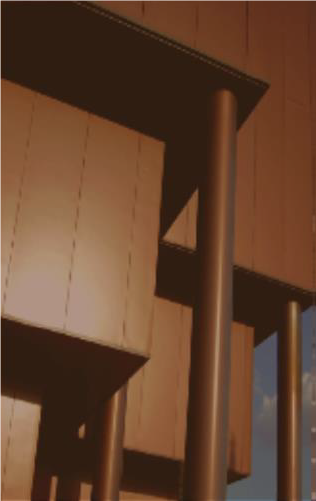
\includegraphics[width=0.7\textwidth]{fig/ilustracion.png}
    \caption{Un ejemplo de ilustración}
    \label{fig:ejemplo}
\end{figure}

Observe que las figuras se numeran automáticamente según el capítulo y el número de figuras que hayan aparecido anteriormente en dicho capítulo. Existen muchas maneras de definir el tamaño de una figura, pero se aconseja utilizar la mostrada en este ejemplo: se define el ancho de la figura como un porcentaje del ancho total de la página, y la altura se escala automáticamente. De esta manera, el ancho máximo de una figura sería 1.0 * textwidth, lo que aseguraría que se muestra al máximo tamaño posible sin sobrepasar los márgenes del documento.

Tenga en cuenta que LaTeX intenta incluir las figuras en el mismo sitio donde se declaran, pero en ocasiones no es posible por motivos de espacio. En esos casos, LaTeX colocará la figura lo más cerca posible de su declaración, puede que en una página diferente. Esto es un comportamiento normal y no debe ser evitado.

\section{Referencias}
Observe cómo en el código fuente de esta sección se ha usado varias veces el comando ``label''. Este comando permite marcar un elemento, ya sea capítulo, sección, figura, etc. para hacer una referencia numérica al mismo. Para referenciar una ``label'' se usa el comando ``ref'' incluyendo el nombre de la referencia:

Este es el capítulo \ref{cap:ejemplos}.

En la sección \ref{sec:estilos} se muestran ejemplos de estilos.

La subsección \ref{sec:subseccion} explica...

En la Figura \ref{fig:ejemplo} vemos que...

Esto evita que tengamos que escribir directamente los índices de las secciones y figuras que queremos mencionar, ya que LaTeX lo hace por nosotros y además se encarga de mantenerlos actualizados en caso de que cambien (pruebe a mover este capítulo al final del documento y observe cómo se actualizan automáticamente todos los índices referenciados). Además, las referencias mediante ``ref'' actúan como hipervínculos dentro del documento que llevan al elemento referenciado al pulsar en ellas.

Es habitual nombrar las ``label'' con un prefijo que indica el tipo de elemento para encontrarlo luego más fácilmente, pero no es obligatorio.

\section{Extractos de código}

Se pueden incluir extractos de código mediante lstlisting:

\begin{lstlisting}[language=Python, caption={Código Python}, label={cod:python}, captionpos=b]
num = float(input("Enter a number: "))
if num > 0:
   print("Positive number")
elif num == 0:
   print("Zero")
else:
   print("Negative number")
\end{lstlisting}

Se admite gran variedad de lenguajes:

\begin{lstlisting}[language=Java, caption={Código Java}, label={cod:java}, captionpos=b]
public class Test {
    public static void main(String[] args) {
        System.out.println("Hello, world!");
    }
}
\end{lstlisting}

Los extractos de código también se pueden referenciar mediante label/ref: Extractos de código \ref{cod:python} y \ref{cod:java}.

\section{Enlaces}
Puede enlazar una web externa mediante el comando url: \url{https://www.example.com}. También se puede vincular un enlace a un texto mediante el comando href: \href{https://www.example.com}{dominio de ejemplo}.

\section{Citas y bibliografía}
En LaTeX, los elementos de la bibliografía se almacenan en un fichero bibliográfico en un formato llamado BibTeX, en el caso de este proyecto se encuentran en ``bibliografia.bib''. Para citar un elemento se usa el comando ``cite''. Se pueden citar tanto artículos científicos \cite{berners1994} o libros \cite{swales1994} como enlaces web \cite{webETSII}. Las citas se numeran automáticamente y se incluyen en la sección de bibliografía del documento.

Observe cómo los elementos bibliográficos almacenados en ``bibliografia.bib'' tienen una etiqueta asociada, que es la que se incluye al citarlos mediante cite. Añadir una referencia al fichero bibliográfico no hace que ésta aparezca automáticamente en la sección de bibliografía del trabajo, es necesario citarla en algún lugar del mismo.

\section{Ecuaciones}
LaTeX tiene un potente motor para mostrar ecuaciones matemáticas y un amplio catálogo de símbolos matemáticos. El entorno matemático se puede activar de muchas maneras. Para incluir ecuaciones simples en un texto se pueden rodear de símbolos dólar: $1 + 2 = 3$, $\sqrt{81} = 3^2 = 9$, $\forall x \in y~\exists~z : S_z < 4$.

Las ecuaciones más complejas pueden expresarse aparte y son numeradas: ecuación \ref{eq:ecuacion}.

\begin{equation}\label{eq:ecuacion}
\lim_{x\to 0}{\frac{e^x-1}{2x}}
 \overset{\left[\frac{0}{0}\right]}{\underset{\mathrm{H}}{=}}
 \lim_{x\to 0}{\frac{e^x}{2}}={\frac{1}{2}}
 +7 \int_0^2
  \left(
    -\frac{1}{4}\left(e^{-4t_1}+e^{4t_1-8}\right)
  \right)\,dt_1
\end{equation}

Dispone \href{http://www.yann-ollivier.org/latex/texsymbols.pdf}{aquí} de un amplio listado de símbolos que pueden usarse en modo matemático.

\section{Caracteres y símbolos especiales}
Algunos caracteres y símbolos deben ser escapados para poder representarse en el documento, ya que tienen un significado especial en LaTeX. Algunos de ellos son:

\begin{itemize}
    \item El símbolo dólar \$ se usa para ecuaciones.
    \item El tanto por ciento \% se usa para comentarios en el código fuente.
    \item El símbolo euro \euro{} suele dar problemas si se escribe directamente.
    \item El guión bajo \_ se usa para subíndices en modo matemático.
    \item Las comillas deben expresarse `así' para comillas simples y ``así'' para comillas dobles. Las comillas españolas pueden expresarse \textquote{así}.
    \item La barra invertida o contrabarra \textbackslash{} se usa para comandos LaTeX.
    \item Otros símbolos que deben escaparse son las llaves \{ \}, el ampersand \&, la almohadilla \# y los símbolos mayor que \textgreater{} y menor que \textless{}.
\end{itemize}
    
    % Bibliografía
    \bibliographystyle{plainnat}
    \bibliography{bibliografia.bib}

% Fin del documento
\end{document}
